% !TEX root = ../thesis_main.tex


% "fig:thechamber"

\begin{figure}[h!!!tb]
	\centering
%	\hspace*{\fill}%
	\subfloat[A decay event within the TRINAT science chamber.  After a decay, the daughter will be unaffected by forces from the MOT.  Positively charged recoils and negatively charged shake-off electrons are pulled towards detectors in opposite directions.  Although the $\beta^+$ is charged, it is also highly relativistic and escapes the electric field with minimal perturbation.
	%\comment{The pic is still kind-of fuzzy.}
	]
	{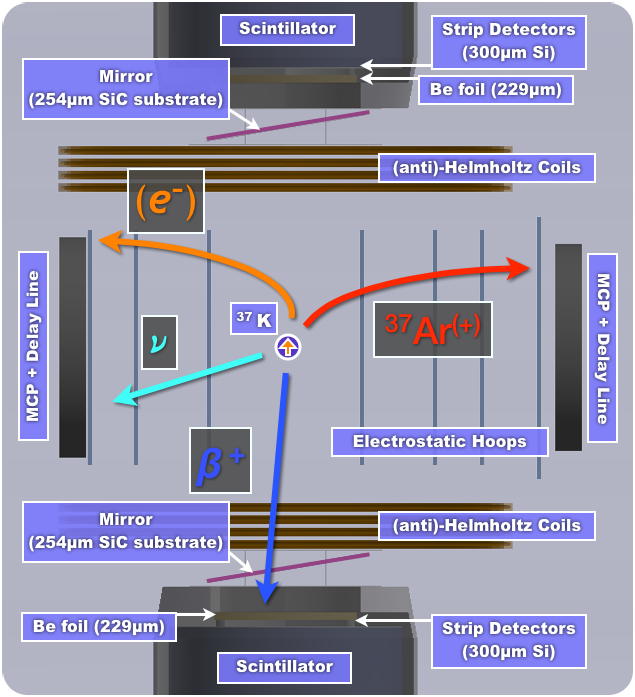
\includegraphics[width=.530\linewidth]{Figures/chamber_decayevent3.png}\label{chamber_decayevent} }
	\hspace*{\fill}
%	\hfill
	\hspace*{\fill}
	\subfloat[Inside the TRINAT science chamber.  This photo is taken from the vantage point of one of the microchannel plates, looking into the chamber towards the second microchannel plate.  The current-carrying copper Helmholtz coils and two beta telescopes are visible at the top and bottom.  The metallic piece near the center is one of the electrostatic `hoops' used to generate an electric field within the chamber.  The hoop's central circular hole allows access to the microchannel plate, and the two elongated holes on the sides allow the MOT's trapping lasers to pass unimpeded at an angle of 45 degress `out of the page'.]	
	{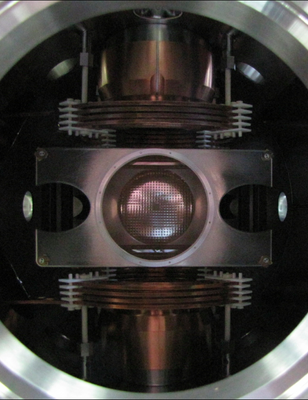
\includegraphics[width=.444\linewidth]{Figures/chamber_photo_2.png}}
%	\hspace*{\fill}%
	\caption{The TRINAT detection chamber}	
	\label{fig:thechamber}
\end{figure}

